\documentclass[UTF8]{ctexart}
\usepackage{amssymb}
\usepackage{pdfpages}
\usepackage{upgreek}

\begin{document}
    \section{密码学概述}
    \subsection{信息安全}
    \begin{itemize}
        \item 计算机网络的建立和普及将彻底改变人类生存和生活模式
        \item 信息化以他有别于传统方式的信息获取、存储、处理、传输和使用, 给现代化社会的正常发展带来了一系列的前所未有的风险和威胁
        \item 传统的一切准则在电子信息环境中如何体现和维护, 到现在并没有根本解决, 一切都在完善中
        \item 今天, 人们一方面享受着信息技术带来的巨大变革, 同时也承受着信息被篡改、泄露、伪造的威胁, 以及计算机病毒及黑客入侵等安全问题. 信息安全的风险制约着信息的有效使用, 并对经济、国防乃至国家的安全构成威胁
        \item 一方面: 没有信息安全, 就没有完全意义上的国家安全. 另一方面: 信息安全还涉及到个人权益、企业生存和金融风险防范等.
        \item 密码技术和管理实信息安全技术的核心, 是实现保密性、完整性、不可否认性的关键.
        \item "911事件"后, 各国政府纷纷站在国家安全的角度把信息安全列入国家战略. 重视对网络信息和内容传播的监控, 更加严格的加固网络安全防线, 把信息安全威胁降到最低限度.
        \item 2000年我国开始着力建立自主的公钥基础设施, 并陆续启动了信息系统安全等级保护和网络身份认证管理服务体系.
        \item 因此, 密码学的基本概念和技术已经成为信息科学工作者知识结构中不可或缺的组成部分.
    \end{itemize}

    \subsection{密码学引论}
    \begin{enumerate}
        \item 密码学的发展概况
        \begin{itemize}
            \item 密码学是一门既古老又年轻的学科.
            \item 自从有了战争, 就有了加密通信. 交战双方都为了自己的通信安全, 窃取对方的情报而研究各种信息加密技术和密码分析技术.
            \item 古代行帮暗语和一些文字游戏等, 实际上就是对信息的加密. 这种加密方法通过原始的约定, 把需要表达的信息限定在一定的范围内流通.
            \item 古典密码主要用于政治、军事及外交等领域.
            \item 电报发明后, 商业方面对密码学的兴趣主要集中在密码本的编制.
            \item 20世纪初期, 集中在机械加密和电动机械加密的设计和制造上.
            \item 进入信息时代, 大量敏感信息要通过公共通信设施或计算机进行交换, 密码学的应用已经不仅仅局限在政治、军事、外交等领域上, 其商业和社会价值日益显著, 并与人们的日常生活紧密相关.
            \item 密码学被当作应用数学和计算机科学的一个分支, 其理论和技术已经得到迅速发展.
        \end{itemize}
        \item 密码学发展的里程碑
        \begin{itemize}
            \item 1949年, 香浓发表了"保密系统的通信理论(Communication Theory of Secrecy Systems)"一文, 为密码学奠定了坚实的理论基础, 使密码学成为一门真正的科学.
            \item 1975年, WD和MEH发表了"密码学中新方向(New Directions in Cryptography)"一文, 提出了一种崭新的密码设计思想, 导致了密码学的一场革命. 首次证明了从发送端到接收端无密钥传输的保密通信的可能, 开创了公钥密码学的新纪元.
            \item 1977年, 美国国家标准局(National Bureau of Standard)正式公布了数据加密标准DES(Data Encryption Standard), 将DES算法公开, 解开了密码学的神秘面纱, 密码学研究进入了一个崭新的时代.
        \end{itemize}
        \item 密码学的基本概念
        \begin{enumerate}
            \item 基本术语
            \begin{itemize}
                \item 明文: 没有加密的信息称为明文(plaintext)
                \item 密文: 加密后的信息被称为密文(ciphertext)
                \item 解密: 从密文到明文的变换被称为解密(decryption)
                \renewcommand{\labelitemi}{\scriptsize$\blacksquare$}
                \item 加密和解密都是在密钥(key)的控制下进行的. 给定一个密钥, 就可确定一对具体的加密变换和解密变换
            \end{itemize}
            \item 密码体制的组成

            \begin{itemize}
                {
                    \renewcommand{\labelitemi}{\scriptsize$\blacksquare$}
                    \item 一个密码体制的组成:
                }
                \item 明文空间M: 全体明文的集合.
                \item 密文空间C: 全体密文的集合.
                \item 密钥空间K: 全体密钥的集合. 通常每个密钥k都有加密密钥$k_e$和解密密钥$k_d$组成, $k=<k_e, k_d>$, $k_e$和$k_d$可能相同也可能不相同.
                \item 加密算法E: 由加密密钥控制的加密变换的集合.
                \item 解密算法D: 由解密密钥控制的解密变换的集合.

                {
                    设$m \in M$是一个明文, $k=<k_e, k_d> \in K$是一个密钥, 则
                    $$c=E_{k_e}(m) \in C$$
                    $$m=D_{k_d}(c) \in M$$
                    其中$E_{k_d}$是由加密密钥确定的加密变换, $D_{k_d}$是由解密密钥确定的解密变换. 在一个密码体制中, 要求解密变换市加密变换的逆变换. 因此, 对任意的$m \in M$都有$D_{k_d}(E_{k_e}(m))=m$成立
                }
                {
                    \renewcommand{\labelitemi}{\scriptsize$\blacksquare$}
                    \item 密钥空间中不同密钥的个数称为密钥量, 他是衡量密码体制安全性的一个重要标准.
                }
            \end{itemize}
            \item 密码体制分类
            \begin{itemize}
                \item 单密钥密码密码体制(对称密码体制): 如果一个密码体制的加密密钥与解密密钥相同, 则称改密码体制为单密钥密码密码体制
                \item 双密钥密码密码体制(非对称密码体制): 如果一个密码体制的加密密钥与解密密钥不相同, 则称该密码体制为双密钥密码密码体制
                \item 公钥密码密码体制(public-key cryptosystem): 在一个双密钥密码密码体制中, 由加密密钥$k_e$计算解密密钥$k_d$是困难的, 公开$k_e$不会损害$k_d$的安全性, 则可以将加密密钥$k_e$公开. 这样的密码体制称为公钥密码体制.
            \end{itemize}
            \item 密码体制的条件

            \begin{itemize}
                {
                    \renewcommand{\labelitemi}{\scriptsize$\blacksquare$}
                    \item 一个好的密码体制至少应该满足以下两个条件:
                }
                \item 在已知明文m和加密密钥$k_e$时, 计算$c=E_{k_e}(m)$容易, 在已知密文c和解密密钥$k_d$市, 计算$m=D_{k_d}(c)$容易.
                \item 在不知解密密钥$k_d$时, 不可能由密文c推知明文m
                {
                    \renewcommand{\labelenumi}{\scriptsize$\blacksquare$}
                    \item 对一个密码体制, 如果能够根据密文确定明文或密钥, 或者能够根据明文和相应的密文确定密钥, 则称这个密码体制是可破译的; 否则, 称其为不可破译的.
                }
            \end{itemize}
            \item 攻击密码体制的方法
            \begin{itemize}
                {
                    \renewcommand{\labelitemi}{\scriptsize$\blacksquare$}
                    \item 密码分析者攻击密码体制的三种主要途径:
                }
                \item 穷举攻击: 密码分析者通过试遍所有的密钥进行破译. ---可以通过增大密钥量来对抗穷举攻击.
                \item 统计分析攻击: 密码分析者通过分析密文和明文的统计规律来破译密码. ---可以通过设法使明文的统计规律与密文的统计特性不同来对抗这种攻击.
                \item 解密变换攻击:密码分析者针对加密变换的数学基础, 通过数学求解的方法来设法找到相应的解密变换. ---可以通过选用具有坚实的数学基础和足够复杂的加密算法对抗这种攻击.

                {
                    \renewcommand{\labelitemi}{\scriptsize$\blacksquare$}
                    \item 密码分析者通常可以在下述四种情况下对密码体制进行攻击:
                }

                \item 唯密文攻击 (ciphertext-only attack): 密码分析者仅知道一些密文
                \item 已知明文攻击 (known-plaintext attack): 密码分析者知道一些明文和相应的密文.
                \item 选择明文攻击 (chosen-plaintext attack): 密码分析者可以选择一些明文, 并得到相应的密文.
                \item 选择密文攻击 (chosen-ciphertext attack): 密码分析者可以选择一些密文, 并得到相应的明文.
                {
                    \renewcommand{\labelitemi}{\scriptsize$\blacksquare$}
                    \item 其中, 唯密文攻击的强度最弱, 其他情况的攻击强度依次增加.
                    \item 绝对不可破译的密码体制: 对一个密码体制, 如果密码分析者无论截获多少密文以及无论用什么样的方法攻击都不能破译, 则称其为绝对不可破一的密码体制. 绝对不可破译的密码体制理论上是存在的.
                    \item 计算上不可破译的密码体制: 是指密码分析者根据可以利用的资源进行破译的时间非常长, 或者破译的时间长到是原来的明文失去保密的价值.
                }
            \end{itemize}

            \item 密码学分成为两个分支:
            \begin{itemize}
                \item 密码编码学: 寻求生成高强度、有效的加密或认证算法
                \item 密码分析学: 破译密码或者伪造加密信息. 分为:
                \begin{itemize}
                    \item 被动攻击: 只是对传输的信息进行窃听; 主动攻击, 对传输的信息采用插入
                    \item 主动攻击: 对传输的信息采取插入、删除、修改、重放、伪造等举动
                \end{itemize}
            \end{itemize}
        \end{enumerate}
    \end{enumerate}

    \subsection{密码应用举例}
    \begin{itemize}
        \item 商品标签形如"ZZ", "QPRA"之类的符号, 代表价格. 选取一个秘密单词(如complexity), 使其与自然对数对应:

            \centering
            \begin{tabular}{|c|c|c|c|c|c|c|c|c|c|} %l(left)居左显示 r(right)居右显示 c居中显示
                \hline
                C&O&M&P&L&E&X&I&T&Y\\
                \hline
                0&1&2&3&4&5&6&7&8&9\\
                \hline
            \end{tabular}

    \end{itemize}

    \subsection{现代密码学的特点}
    \begin{itemize}
        \item 有坚实的理论基础, 已经形成一门新的科学;
        \item 对密码学公开的研究;
        \item 应用于社会各个方面;
        \item 破译密码系统归结为求解数学的难题问题.
    \end{itemize}

    总结几百年密码学研究的成果可以得出以下几条研究和发展密码学的经验:
    \begin{itemize}
        \item 不应该低估对手的能力;
        \item 只有密码分析者才能评价一个密码体制的安全性. 同时, 每个涉及安全密码体制的机构也应该有破译"认为是安全的密码体制" 的任务;
        \item 对手知道所用的密码体制
        \item 表面上的复杂性可能是虚假的, 虽然他们可能给密码编译者一种安全性的错觉
        \item 由于人自身的弱点, 会发生密码错误和其他违反安全纪的情况. 判断一类方法的安全性时, 必须考虑这点.
    \end{itemize}

    \subsection{对称密钥加密}
    对称密钥加密是指密码方案中, 从加密密钥容易计算出解密密钥或反过来从解密密钥容易计算出加密密钥. 对称密钥加密也称单钥加密或传统加密, 其加密和解密经复杂的线性变换实现, 对称密钥加密技术包括分组密码和序列密码

    \begin{itemize}
        \item 分组密码
        \begin{itemize}
            {
                \renewcommand{\labelitemi}{\scriptsize$\blacksquare$}
                \item 分组密码是在定长的块上进行替代操作, 换位操作或者他们的合成(乘法加密).
            }
            \item 替代: 是将明文中的一个字母用文字母表中其他字母替代.
            \item 换位: 是一块中的字母简单的置换.
            {
                \renewcommand{\labelitemi}{\scriptsize$\blacksquare$}
                \item 分组密码目前广泛运用于数据的保密传输和存储加密.
            }
        \end{itemize}
        \item 序列密码
            序列密码和加密变换只改变一位明文, 固他就可以看成是块长度为1的分组密码

            序列密码是各国军事和外交等领域使用的主要密码体制. 其主要问题是如何使生成的密钥流周期长、复杂度高, 随机性特性足够好, 使之尽可能地接近一次一密的密码体制.

            对称密码的优缺点:
            \begin{itemize}
                \item \underline{对称密钥密码的优点}:
                \begin{itemize}
                    \item 加密效率高, 硬件实现可达没秒数百兆字节(软件实现略慢一些).
                    \item 密钥相对比较短.
                    \item 可以用来构造各种密码体制.
                    \item 可以用来建造安全性更强的密码.
                \end{itemize}
                \item \underline{对称密钥密码的缺点}:
                \begin{itemize}
                    \item 通信双方都要保持密钥的秘密性;
                    \item 在大型网络中, 每个人需持有许多密钥;
                    \item 为了安全, 需要经常更换密钥
                \end{itemize}
            \end{itemize}
            \item
        \end{itemize}

    \subsection{数字签名、认证与识别}
    \begin{enumerate}
        \item 数字签名
            数字签名是把实体和一段信息捆绑在一起的一种手段. 它包括签名过程和验证过程.

            数字签名要求:
            \begin{itemize}
                \item 每个用户都能有效的为他的特定消息生成签名;
                \item 每个用户都能有效地验证是否是特定人对特定消息的签名;
                \item 任何人不能有效地生成他人对特定消息的签名并且通过验证过程
                {
                    \renewcommand{\labelitemi}{\scriptsize$\blacksquare$}
                    \item 1991年出现了第一个基于RSA公钥签名方案的数字签名国际标准.
                }
            \end{itemize}
            \item 认证与识别
                认证就是保证"实体是他所声称的那个实体" 或 "某个信息没有收到非授权实体的处理" 的一种手段.

                根据是狗需要实时地相互交换信息认证分为识别和数据源认证. 前者双方通信是实时的, 后者是有时间延迟的.

                数据源认证要求:
                \begin{itemize}
                    \item 通信双方都能为自己发送的特定消息生成一个认证标记;
                    \item 通信双方都能有效地验证此标记是该消息地认证标记;
                    \item 第三者不能对通信双方发送的消息产生认证标记.
                \end{itemize}
    \end{enumerate}

    \subsection{公钥密码学}
        1976年WD和MEH的文章引入了公钥密码学的概念, 给出了一种新的密钥交换方法, 这种方法的安全性基于离散对数问题的难解性.

        1978年出现了第一个基于大整数素因子分解难题问题的RSA公钥加密签名方案.

        1985年出现了一个基于离散对数问题的ElGamal公钥加密方案.

        \begin{itemize}
            \item 公钥加密
            公钥加密方案$E_e$和解密方案$D_d$中, 对于每对加密密钥e和解密密钥d, 其中加密密钥(公钥)是公开的, 而解密密钥(私钥)只为一个实体私有.

            公钥加密的优缺点:

            \begin{itemize}
                \item \underline{公钥加密的优点}:
                \begin{itemize}
                    \item 在大型网络中, 每个用户需要的密钥数量少;
                    \item 对管理公钥的可信第三方信任程度要求不高而且是离线的;
                    \item 只有私钥是保密的, 而公钥只要保证他的真实性.
                \end{itemize}
                \item \underline{公钥加密的缺点}:
                \begin{itemize}
                    \item 多数公钥加密比对称密钥加密的速度慢几个数量级;
                    \item 公钥加密方案的密钥长度比对称密钥加密的密钥长;
                    \item 公钥加密方案没有被证明是安全的.
                \end{itemize}
            \end{itemize}
        \end{itemize}

    \section{密码协议与密码机制}
        在密钥建立、密钥分配、身份识别中, 需使用加密、数字签名、哈希函数、随机数生成等基本原语. 把使用密码学基本原语的分布式算法特别称为密码协议.

        为达到某种安全目的所需的各种手段(包括协议、算法以及非密码的技术)构成密码机制.

        对手可能在没有攻破密码原始原语的情况下, 从密码协议或密码机制得到好处, 则称\underline{密码协议或密码机制失败}. 这是因为密码协议或密码机制\underline{扩大了原语的弱点}或\underline{没有准确理解所声称的安全性}.

    \section{攻击分类与安全模式}
        在密码系统所处中的环境中除发送者、接收者之外, 还有\underline{攻击者}. 攻击者通过各种方法窃听和干扰信息.

        窃听信息称为\underline{被动攻击}, 手段是\underline{电磁侦听}或\underline{搭线窃听}, 主要破坏信息的\underline{保密性}.

        干扰信息称为\underline{主动攻击}, 通过\underline{删除}、\underline{更改}、\underline{插入}、\underline{重放}、\underline{伪装}等方法向系统注入信息, 主要\underline{破坏信息的完整性}.

        {
            \centering
            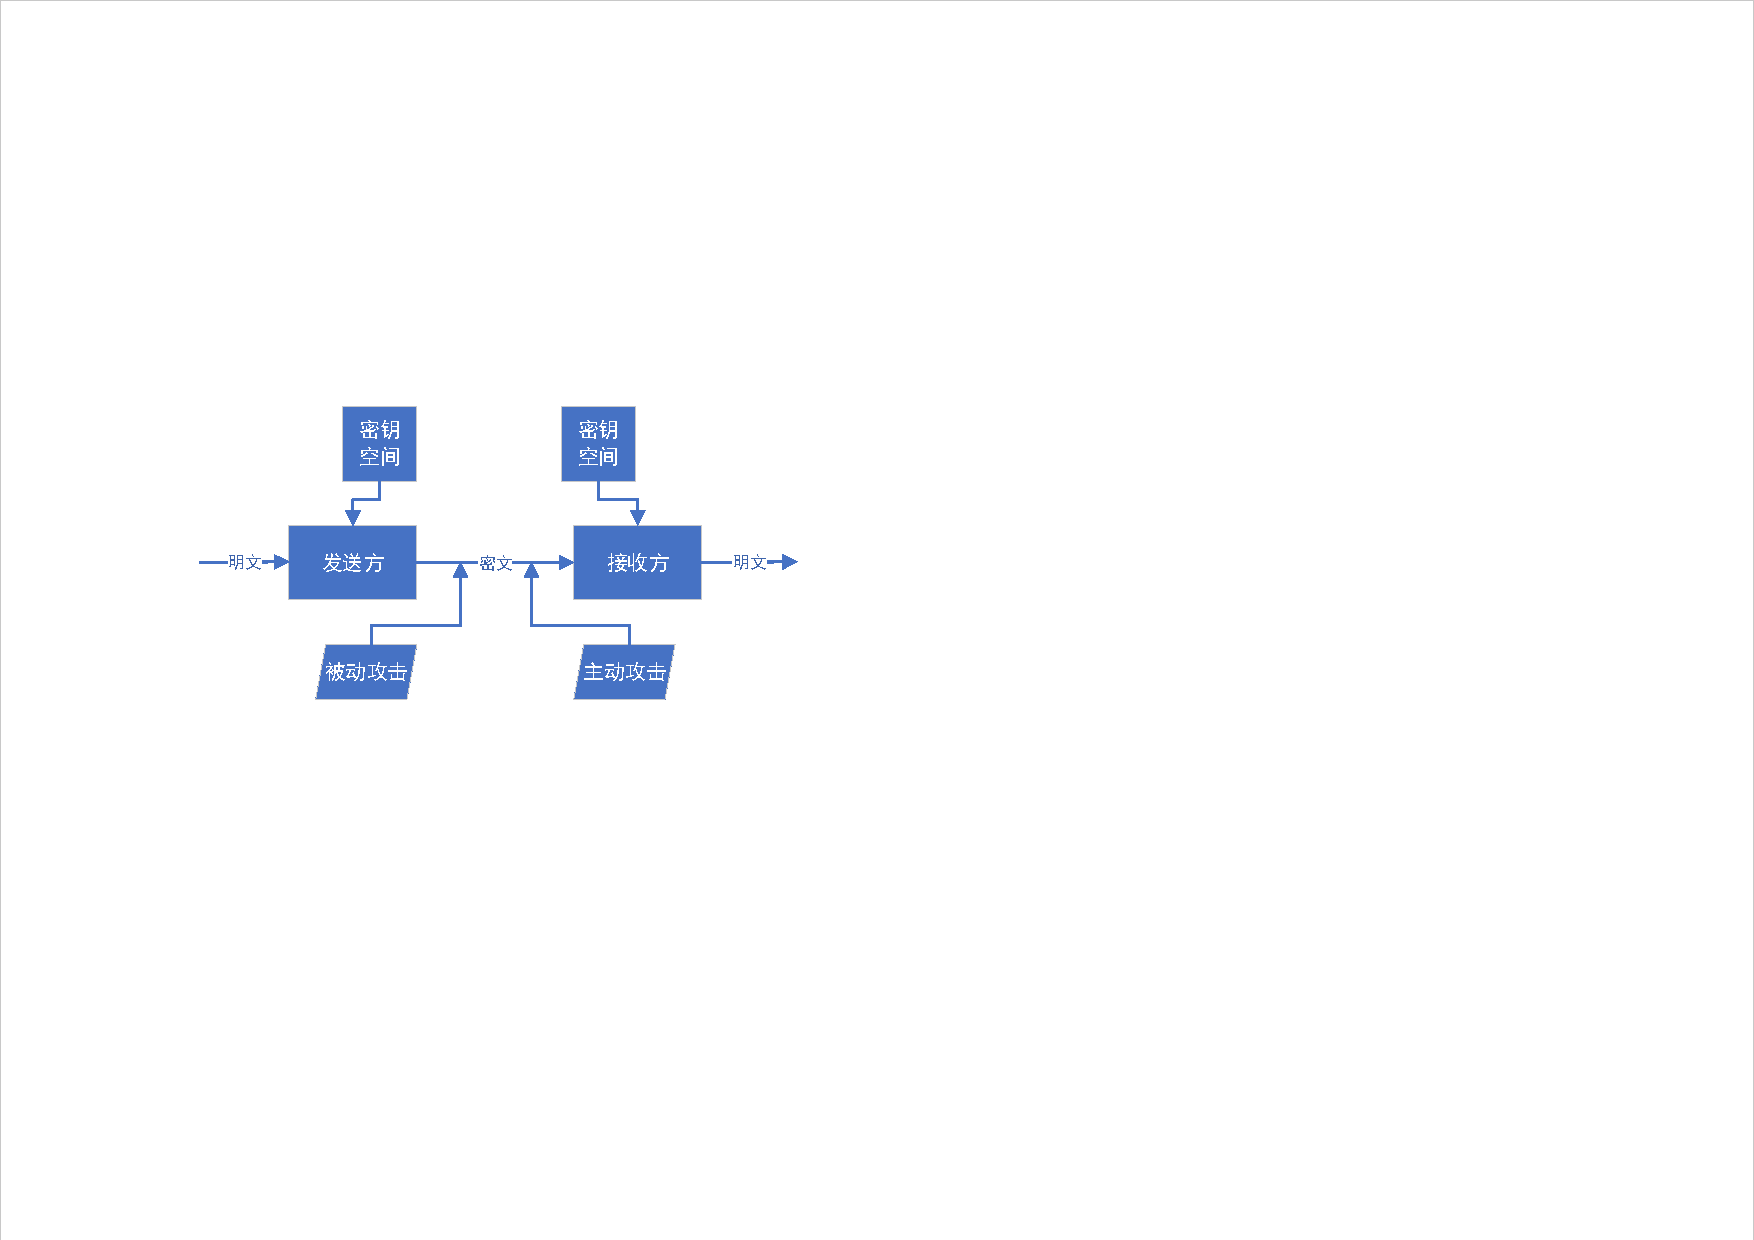
\includepdf[pages={1}, width=2\textwidth]{p11.pdf}
        }

        从攻击的对象分, 既可以是加密算法, 也可以是密码协议

        \begin{itemize}
            \item 对加密算法的攻击
            根据分析者使用的数据不同, 主要有:
            \begin{itemize}
                \item 仅有密文攻击: 密码分析者仅根据截获的密文来破译密码;
                \item 已知明文攻击: 密码分析者根据一致的某些明文-密文对来破译密码;
                \item 选择明文攻击: 密码分析者能够选择明文并获得相应的密文.
            \end{itemize}
            \item 对密码协议的攻击
            主要有:
            \begin{itemize}
                \item 已知密钥攻击: 对手从用户以前的用过的密钥确定出新的密钥;
                \item 重放攻击: 对手记录一次通信会话, 在以后的某个时候重新发送整个或部分会话;
                \item 伪装攻击: 对手扮演网络中的一个合法的实体.
                \item 字典攻击: 主要针对口令的一种攻击.
            \end{itemize}

            \item 安全模式
            密码学原语和密码协议的安全性可以有不同的评估模型: 无条件安全性、可证明安全性和计算安全性.
            \begin{itemize}
                \item \underline{无条件安全性}: 即使在无限计算条件下, 通过观察密文也不会为对手提供任何有助于破译密码的信息;
                \item \underline{可证明安全性}: 如果能证明挫败一个密码学方法跟某个著名的的困难问题的困难程度相同, 则称这个密码学方法是可证明安全的;
                \item \underline{计算安全性}: 某种方法是计算安全的, 是指使用当前最好的方法攻破它的计算远远超过对手的计算资源水平.
            \end{itemize}
        \end{itemize}

    \section{复杂性理论}
    计算复杂性理论是密码分析技术中分析计算需求和研究破译密码的的固有难度的基础. 密码强度由破译改密码所用的算法和的计算复杂度决定.

    算法的计算复杂性理论由他所需要的\underline{时间量级}和\underline{空间量级}来度量
    \begin{itemize}
        \item 独立于所用的系统
        \item 使人们看到时间和空间的需求随输入规模n的增长而增长
    \end{itemize}
    通常使用时间或空间复杂性对算法进行分类. 若对某个常数t, 常熟的运行时间$T=O(n^t)$, 则称该算法是\underline{多项式时间}的.

    若对某个常数t和多项式$h(n)$, 算法的运行时间$T=O(t^{h(n)})$, 则称该算法是\underline{指数时间}的.

    \centering
    \begin{tabular}{c|c|c|c} %l(left)居左显示 r(right)居右显示 c居中显示
        \hline
        算法类型& 复杂度& 操作次数& 时间需求\\
        \hline
        常数的& $O(1)$& 1& $1\upmu$s\\
        线性的& $O(n)$& $10^6$& 1s\\
        二次方的& $O(n^2)$& $10^{12}$& 11.6d\\
        三次方的& $O(n^3)$& $10^{18}$& 3200y\\
        指数的& $O(2^n)$& $10^{30130}$& $3*10^{30130}$y\\
        \hline
    \end{tabular}
\end{document}